% \documentclass[a4paper,11pt]{article}

\documentclass{article}

\usepackage{subcaption}

% \documentclass[varwidth, border=10pt]{standalone}
% border={10pt 5pt} % left/right bottom/top
% border={20pt 20pt 0pt 20pt} % left right bottom top
% \documentclass[11pt]{article}
% \documentclass[
%     a4paper, aps,floatfix, superscriptaddress,
%     nofootinbib]{revtex4-1}

\usepackage[utf8]{inputenc}
\usepackage[load=addn]{siunitx}
\usepackage[english]{babel}
\usepackage[document]{ragged2e}
\usepackage{amsmath}
\usepackage{amssymb}
% \usepackage{graphicx}
\usepackage{float}
\usepackage{biblatex}

\usepackage{listings}
\usepackage{pgfplotstable}
\usepackage{booktabs}

\usepackage{multirow}
\usepackage{booktabs}

\usepackage{subcaption}
\usepackage[labelformat=parens,labelsep=quad,skip=3pt]{caption}
\usepackage{graphicx}
\usepackage{svg}
\usepackage{geometry}



% \usepackage{indentfirst}

% Colour scheme, see https://tex.stackexchange.com/a/119184/128247
\usepgfplotslibrary{colorbrewer}
\pgfplotsset{cycle list/Dark2}

\pgfplotstableset{
    every head row/.style={before row=\toprule,after row=\midrule},
    every last row/.style={after row=\bottomrule}
}

{\setlength\doublerulesep{5pt}}   %%<-- sep between consecutive rules

\addbibresource{references.bib}



% \title{FYS5555 Project 2}
% \author{fosheimdet }
% \date{April 2020}

\begin{document}

{\setlength\doublerulesep{5pt}}   %%<-- sep between consecutive rules

\begin{titlepage}

\title{Search for High Mass Dilepton Resonances Using $\SI{10.6}{\femto\barn}^{-1}$ of Open Atlas Data at $\sqrt{s} = \SI{13}{\tera \eV}$ }
\author{Håkon Fossheim}
\date{\href{https://github.com/fosheimdet/FYS5555/tree/master/Project3}{}}
\maketitle


\newcommand{\HRule}{\rule{\linewidth}{0.5mm}} % Defines a new command for the horizontal lines, change thickness here

%\center % Center everything on the page

% \begin{enumerate}
%     \item Irreducible(Drell Yan) and reducible processes (A story article). The Drell Yan consitute the main background, but because its important to asses the contribution of reducible SM processes. [cite a story]
    
%     The main background from reducible processes are  $t\Bar{t}$, W+jets, Z+jets, multijets and diboson processes such as WW, WZ and ZZ [find Feynman diagrams].  
    
%     \item One reason to include missing transverse energy: 
%     In the W+jets background we may e.g. have a W+ decaying to a lepton and a neutrino. Another source of missing energy might be the failure to detect a particle. 
% \end{enumerate}


\section{Introduction}

The standard model is to date our best description of reality. It paints a picture of four fundamental forces: electromagnetism, the weak force, the strong force and gravity. So far, the force carries for all the forces have all been discovered except the hypothetical graviton, thought to mediate the gravitational force. 
Although the standard model has been immensely successful, it cannot be the final description of reality as it stands. One reminder of this is the fact that the angular momentum of galaxies is far to great to hold them together if not for some unknown form of matter holding them together, aptly coined dark matter. Furthermore, there is no consensus for why the forces should differ so immensely in strength, e.g. why the weak force is $10^{24}$ times stronger then gravity. This is referred to as the hierarchy problem. In addition, the weak force violates charge-parity symmetry by coupling only to left handed chiral particles and right handed chiral anti-particles.  

Grand Unified Theories (GUTS) seek to solve some of these problems by unifying electromagnetism, the weak force and the strong force to a single gauge group. Excluding gravity is what demotes these theories from being theories of everything. 

Similarly to how the electromagnetic and weak interaction unify to a single interaction (the electroweak interaction) at high energy scales, GUTS predict the same to happen for the three aforementioned forces at even higher energies. 

Many of these models depend on as-of-yet undiscovered weak bosons, coined the $W'$ and $Z'$ bosons. Their specific properties differ depending on the model. The commonly searched for $Z'$ bosons are the ones belonging to E6-motivated and minimal models. 

The sequential standard model includes a $Z'_{SSM}$ boson which couples to fermions in the same manner as the $Z$ boson. Due to its simplicity, this boson proves useful as a benchmark model and is the one we aim this search at.

% Many Beyond Standard Models predict dilepton resonances in the high invariant mass region. Among these models are the Grand Unified Theories (GUTS), which seek to unify the current gauge theories of the standard model into one gauge group. 

% ///
% In this project, we study the sequential standard model Z prime boson. It is assumed to couple in the same way as the standard model Z. 
% //

\section{Detection of particle collisions in ATLAS}

Rather than colliding two individual protons at a time, which would produce extremely few events, bunches of protons are sent at each other with \SI{25}{\nano \second} intervals at the LHC. Each bunch consists of 110 billion protons. The frequency of the bunch crossings and the number of protons contained in them determines the luminosity ($L$) of the particle accelerator. Events which are not of interest and that are produced in pp collisions within the current or previous bunch crossings are referred to as pileup. Another important factor, aside from the luminosity, is the centre-of-mass energy $\sqrt{s}$, which is a measurement of how much of the energy in the collisions that is available for particle production. In a fixed-target particle accelerator where only one of the particles are accelerated, the final products of the collision must have the same momentum as that of the incoming particle. This restricts the mass of the end products. In the LHC the colliding protons have net zero momentum\footnote{But the colliding partons may not.} and so in principle all of the available energy of the colliding partons could be turned into one massive particle with no momentum, which is not the case in fixed-target colliders.


The ATLAS detector has a cylindrical shape, referred to as the barrel region, which is centered around the beam pipe. It also has two flat end caps, which in conjunction with the barrel region provide almost solid angle coverage around the collision point within the beam pipe. 


A solenoid magnet provide a strong magnetic field in the inner layer of the detector. The field lines are parallel to the beam line and therefore make charged particles follow curved paths in the transverse plane. If the momentum of the particle is not too high, both the charge and momentum can be discerned from the radius and bending direction of the trajectory. 

Surrounding this tracking volume are the electromagnetic and hadronic calorimeters followed lastly by the muon solenoid which provide identification for muons which unlike the vast majority of particles pass through both calorimeters, depositing only ionization energy. 

And so the momenta and charge of particles are determined by the tracking detector, which together with the energy measurments of the calorimeters provide means of identifying particles. 

When electrons hit the EM calorimeter, they create electromagnetic showers which are largely contained in said calorimeter due to dense scintillator material which reduces the mean free path of the shower particles. The electron energy can then be measured based on the size of the shower. Photons are identified as isolated energy deposits within the EM calorimeter\cite{Thomson}.  

Together with the hadron calorimeter which measures the energy of neutral hadrons, the ATLAS detector can measure every particle except neutrinos, which escape undetected. Their existence can however be inferred from momentum conservation. Because the colliding partons have no transverse momenta, the sum of the transverse momenta of all particles produces should be zero. Missing transverse momenta/energy may therefore stem from a neutrino or perhaps a particle which should have been detected, but somehow managed to escape detection. 

Throughout this article we will use a right handed coordinate system with the Z-axis aligned with the beam axis. The angle between a particle's position and the z-axis is given by $\theta$, which is related to the pseudo-rapidity\footnote{Defined as $\eta = -\ln \left[\tan(\theta/2)]$ because differences in this quantity are invariant under Lorentz boosts and so the total observed rapidity difference in the end products are the same as in the colliding quarks.}, $\eta$, of the particle. Furthermore, the transverse direction is specified by $\phi$, which is the angle the particle makes with the x-axis in the xy-plane, viz. transverse plane.

The size of jets are specified by the parameter $\Delta R = \sqrt{(\Delta \eta)^2 + (\Delta \phi)^2}$, which is a measure of the solid angle spanned by the jet and is a constant along the jet axis.

% Surrounding this tracking volume is the electromagnetic calorimeter. It is in essence a scintillator material in order to reduce the size of the 

% The inner most layer of the detector is filled with a strong magnetic field provided by toroidal magnets which is aligned with the beam line. It is provided by so




\section{Event Selection}\label{sec:event_selection}
% We require two or more leptons of the same flavour to be present in the event. The criteria for these leptons are as follows:



% If there are more than two leptons of the same flavour, we pick the two same flavour leptons with the highest $E_T$ in the case of electrons and $p_T$ in the case of muons. This stems from the fact that the electron mass can be neglected at these energies, $E_T \approx p_T$. Note that by "pick", we refer to how we choose to categorize the event. 

% Furthermore, a pair of muons are required to be oppositely charged whilst both same- and oppositely charged electrons are kept due to the increased chance of miss identifying the charge of high $E_T$ electrons. 

% In the case that we get both an electron- and a muon pair, the event is classified as belonging to the ee channel because of the better resolution and higher efficiency for electrons. 

% Lastly, in order to circumvent the Z-boson peak region, the reconstructed mass of the dilepton system ($m_{ll}$ is required to be above \SI{110}{\giga \eV}.

% % $|\eta| > 2.5$ from article. From MySelector: Electon: $|\eta| > 2.47$, muon: $|\eta|$ > 2.4
% /////////////////////////

% The main background of this search 

The event selection of this search is largely based on \cite{mainArt}, but with looser selection criteria as we have less data. The events must satisfy the following: 

\begin{enumerate}
    \item Require exactly two leptons of opposite charge and same flavour
    
    \item Isolation requirements:  Jets may be misidentified as leptons, or correctly identified leptons may stem from hadronic decays within jets. To filter out these scenarios, the leptons are required to be isolated. To ensure this, the $E_T$ sum of good-quality tracks in a cone of $\Delta R = 0.20$ around the lepton candidate must be less than 20\% of the lepton $p_T$. The lepton candidate is excluded from this sum. 
    
   \item Leptons may be categorized as being either \textit{promt} or \textit{non-promt}. \textit{Promt} leptons stem from a hard scattering process in the original collision and are the decay products of heavy, short-lived particles such as the W and Z boson. As such, their vertex have a very small displacement relative to the primary vertex. \textit{Non-promt} leptons stem from heavy flavour jets who's lifetimes are much greater. A relevant example is the b-quark decaying leptonically within a jet. Due to its mass, the leptons stemming from a b-quark decay within a jet may be produced with sufficient momenta in the direction transverse to the jet axis so as to offset their trajectories. Isolation criteria are therefore not sufficient to exclude these leptons. 
   
   We must also require that lepton candidate tracks be consistent with the primary vertex. This is done by essentially restricting how much the lepton vertex is allowed to deviate from the primary vertex in the longitudinal and transverse directions: 
  
    \begin{itemize}
     \item   The longitudinal impact parameter $Z_0$ is required to satisfy $|Z_0 \sin \theta| < \SI{0.5}{\milli \meter}$. The reason we multiply by $\sin \theta$ is that the impact parameter will be greater at smaller angles for tracks originating from the primary vertex, and so we offset this via $\sin \theta$. 
     \item    The transverse impact parameter $d_0$ is the lepton track's point of closest approach to the beamline \footnote{Prior to 2015 $d_0$ was calculated with respect to the position of the primary vertex.}, i.e. its the transverse displacement. One may alternatively measure the transverse displacement by use of the impact parameter significance, defined as $|d_0/\sigma_{d_0}|$ with $d\sigma_{d_0}$ being defined by the error matrix of the track fit\cite{Brendlinger} . We require this ratio to be smaller than 3 for events to pass our selection.
   \end{itemize}
   
   \item  Avoid endcap- and endcap-barrel transition regions of the EM calorimiter due to their reduced precision. Leptons within the corresponding pseudo-rapidity regions are therefore excluded: 
      \begin{itemize}
     \item electrons: $|\eta| < 2.47$ and $1.37 < |\eta| < 1.52$
     \item muons: $|\eta| < 2.5$ and $1.01 < |\eta| < 1.1$
   \end{itemize}
   
  \item Lastly, in order to circumvent the Z-boson resonance peak, the reconstructed mass of the dilepton system ($m_{ll}$) is required to be above \SI{110}{\giga \eV}.
\end{enumerate}

% \begin{itemize}
%   \item Avoid endcap in both channels: $|\eta| > 2.5$
%   \item Avoid barrel endcap transition region in EM calirometer (electrons only): $1.37 < |\eta| < 1.52$
%   \item 
% \end{itemize}




% /////////
% The signal efficiency $\epsilon_{sig}$ is the ratio of number of events after the analysis cut to the number of events before
% ////


\section{Statistical Analysis}



% The dotted lines in figure ... show the exclusion limit $s_{up}$ for every Z' mass. 
 \subsection{Bayesian Inference}\label{sec:Bayes}
Bayesian inference, which we will use to determine our exclusion limits, differs quite a lot conceptually to the frequentist formulation. The main idea in the frequentist approach is to study how likely it is to get the observed number of events under a background- and signal+background hypothesis and thus how confidently we can reject either one of these, which respectively constitutes a discovery or exclusion. 


In the Bayesian formulation, we consider the set of all possible values the signal yield can have as well as the set of all $n_{obs}$ one could measure. Let this be denoted by the stochastic variables $s'$ and $n_{obs}'$ respectively. Mapping the two-dimensional space spanned by these variables to a unit square gives figure \ref{fig:Bayes}, in which the possible outcomes are placed in the shown rectangles which have areas equal to their probabilities (not drawn to scale).  

\begin{figure}[H]
    \begin{center}
        \includesvg[scale=0.6]{Bayes2.svg}
        \caption{Visual depiction of Baye's theorem applied to our analysis.}
        \label{fig:Bayes}
     \end{center}
\end{figure}

What we are really interested in finding is the probability of getting a specific signal yield $s$, given that the number of observed events is $n_{obs}$, namely $P(s'=s|n_{obs}'=n_{obs})$. This can be thought of as the probability of getting the specific signal yield ($P(s'=s)$), represented by the combined blue and purple area times the fraction of these events that have our specific number of observed events. This fraction can be found by looking at the combined red and purple area. As seen, it is given by the probability of getting a signal yield $s$ with $n_{obs}$ observed events given that the number of observed events is $n_{obs}$ ($P(n_{obs}'=n_{obs}|s'=s)$) divided by the probability of observing $n_{obs}$ events, i.e. the ratio of the purple area to the combined purple and red area. 

We therefore have 

\begin{equation}
    P(s'=s|n_{obs}'=n_{obs}) = P(s'=s) \cdot \frac{P(n_{obs}' = n_{obs}|s'=s)}{P(n_{obs}' = n_{obs})}
\end{equation}

Which, if we drop the stochastic variable notation, can be written in the familiar form 

\begin{equation}
    P(s|n_{obs}) = \frac{P(n_{obs}|s) P(s)}{P(n_{obs})}
\end{equation}

Here $P(s|n_{obs})$ is the so-called posterior distribution, so named because it is the our estimate of the probability of getting $s$ after our prior estimate/belief, $P(s)$, has been updated with new evidence, namely the number of observed events. The prior is often set to a flat distribution (i.e. $P(s)$ is a constant) to reflect our lack of knowledge of the process we're searching for.  $P(n_{obs}|s)$ is a binomial distribution with 
\begin{equation}
    P(n_{obs}|s) = \binom{N}{n_{obs}} p^{n_{obs}}(1-p)^{n-n_{obs}}
\end{equation}

Where $N$ are the total number bunch crossing of our search (not just those that are triggered as events), and $n_{obs}$ are the number of those that give events which pass the detector triggers and our analysis cuts. There is a fixed probability of any given event being categorized as an observed event if the true signal yield is $s$, namely $p$. We can show that in the limit as $N$ goes to infinity and $p$ goes to zero, while the number of expected observed events $\lambda = N\cdot p$ remains fixed, this distribution approaches a Poisson distribution, given by 

\begin{equation}
    P(n_{obs}|s) = \frac{\lambda^{n_{obs}} e^{-\lambda}}{n_{obs}!}
\end{equation}

Which we call our likelihood function. Rather than using $\lambda = N\cdot p$, we can estimate the expected number of events if the true signal yield is $s$ through Monte-Carlo simulation of the signal and background: $\lambda = b + s$. 

Lastly, $P(n_{obs})$ is independent of $s$ and so can be absorbed with $P(s)$ and $n_{obs}!$ to a single constant in front of the likelihood function: 

\begin{equation}
    P(n_{obs}|s) = C (s+b)^{n_{obs}} e^{-(s+b)}
\end{equation}

Now we have what we need to calculate exclusion limits. 

The exclusion limit is defined as the signal strength, $s_{up$, above which there is only a 5\% chance to observe $N_{obs}$ events if the true signal actually is greater than or equal to $s_{up}$, for a given number of background events. 

It is found by integrating the posterior distribution in the following manner: 
\begin{equation}\label{eq:s_up}
    \int_{0}^{s_{up}} P(s|n_{obs}) ds = 0.95
\end{equation}

 The only parameters we can have any effect on are the number of observed events and the background. The number of observed events depends both on the trigger conditions of the detector and the cuts we perform in our analysis\footnote{Which consists of event selection and which histogram cuts.}. Once we have decided on the optimal analysis cuts, the only source of potential concern regarding the final exclusion limit comes from the background. 
 
 The background is estimated through Monte-Carlo simulations and has an uncertainty associated with it. We can model the background as being normally distributed with an expectation value equal to the single bin count of the background generated for our analysis, $\Bar{b}$, with a standard deviation of $\delta b$. 
 
 We therefore have to adjust the posterior with a term that takes this into account. We now get a joint posterior distribution, given by 

\begin{equation}
    P(n_{obs}|s,b) =\frac{P(n_{obs}|s) P(s) P(b)}{P(n_{obs})} = C (s+b)^{n_{obs}} e^{-(s+b)} e^{-\frac{(b-\bar{b})^2}{2(\delta b)^2}}
\end{equation}

We now need to integrate out the $b$ variable, viz. marginalize the joint posterior to obtain $P(n_{obs}|s)$. The upper limit for a given $n_{obs}$ can then be found by solving equation \ref{eq:s_up}. We can be shown that if $n_{obs} = 0$, the upper limit is $s_{up} = -\ln{0.05} \approx 3$.
 
 Now, if the final upper limits seem suspiciously high or low compared to e.g. work done by others, and we are confident we have the optimal analysis cuts, then we should be sceptical of the simulated background. To quantify how likely it is that the background indeed is the cause for say an exceptionally strong, viz. low, exclusion limit rather than our peers being wrong, we can do "pseudo-experiments". 
 
 Each pseudo-experiment is set to a background which is a certain (continuous) number of standard deviations from the background of the main experiment ($\Bar{b}$). We can find $s_{up}$ in each of these experiments, and color code those that stem from deviations of $1 \sigma$ or less as green and those that stem from $2 \sigma$ or less as yellow. Doing this for each Z' mass yields figure \ref{fig:exclusion_limits} , from which one can assess how trustworthy the results (the circular dots) are.
 
 
%  to change in the posterior are the number of events and the background.

\subsection{Histogram cuts}\label{sec:histogram_cuts}

The goal of our analysis is to determine whether the number of observed events is consistent with a hypothetical Z' resonance peak and how confident we are in excluding theories which predict this signal yield. 

In principle, could have made no cuts at all. We could have looked at every event triggered by the ATLAS detector during run II and made our single bin span as large as possible.

The reason this is suboptimal is the large "background" this would include. The ratio $\frac{\delta b}{\Bar{b}}$ stays the same, and thus the uncertainty in background in terms of number of events increases. The excess in predicted signal events compared to background would remain the same. To exclude an excess in observed data as not stemming from the background uncertainty, the hypothetical signal yield would have to be very large. In effect, our exclusion limit increases. 
\vspace{5mm}

We therefore try to reduce the background as much as possible through proper event selection and also by restricting our single-bin to a region of the histogram with comparatively high signal to background ratio whilst including most of the potential signal events. Now the uncertainty in the number of background events becomes smaller relative to the expected excess signal yield, and so we can set the exclusion limit lower. 

When choosing the single-bin region in the histogram, the cuts were chosen to minimize the exclusion limit whilst keeping as much of the resonance peak as possible. 


% \begin{figure}
%   \begin{subfigure}{6cm}
%     \centering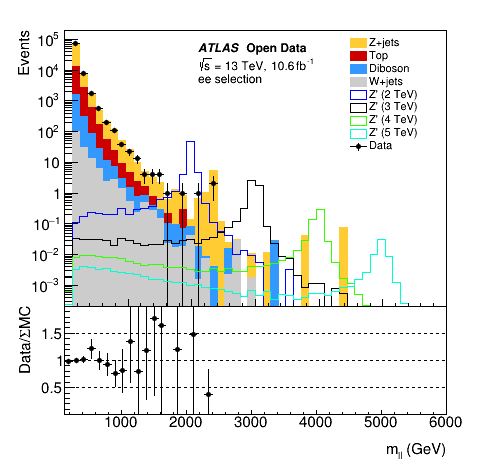
\includegraphics[width=5cm]{ee_mll.png}
%     \caption{Caption text 1}
%   \end{subfigure}
%   \begin{subfigure}{6cm}
%     \centering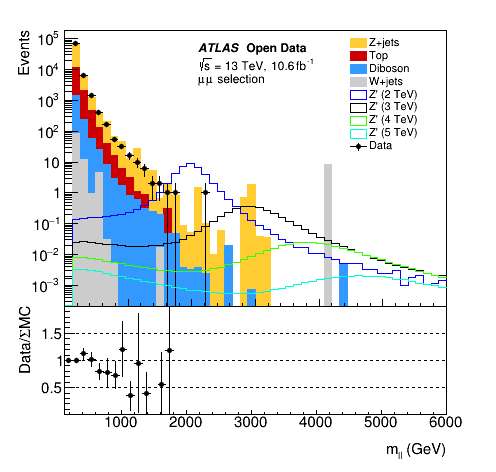
\includegraphics[width=5cm]{uu_mll.png}
%     \caption{Caption text 2}
%   \end{subfigure}
% \end{figure}

% \begin{figure}
% \begin{subfigure}{.6\textwidth}
%   \centering
%   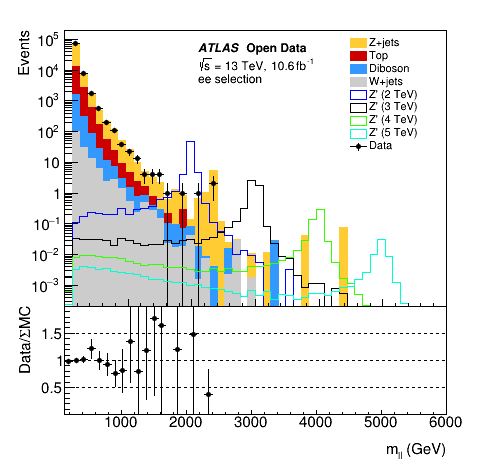
\includegraphics[width=.9\linewidth]{ee_mll.png}
%   \caption{1a}
%   \label{fig:sfig1}
% \end{subfigure}%
% \begin{subfigure}{.6\textwidth}
%   \centering
%   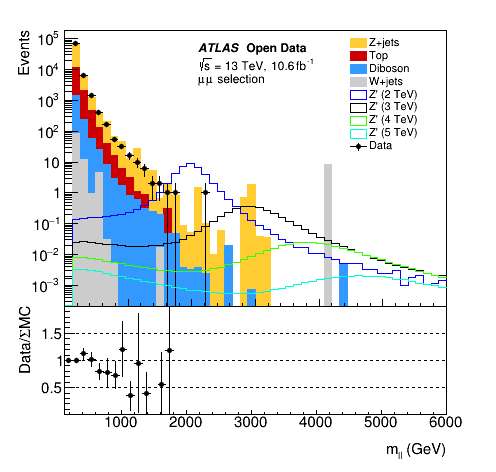
\includegraphics[width=.9\linewidth]{uu_mll.png}
%   \caption{1b}
%   \label{fig:sfig2}
% \end{subfigure}
% \caption{plots of....}
% \label{fig:fig}
% \end{figure}

% \newgeometry{left=2cm,bottom=0.1cm}
% \begin{figure}[H]
% \begin{subfigure}{.5\textwidth}
%   \centering
%   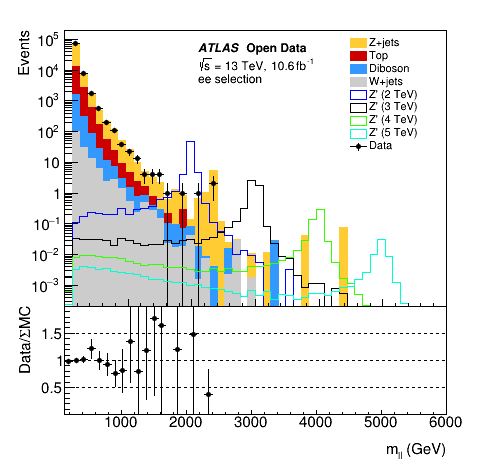
\includegraphics[width=1\linewidth]{ee_mll.png}
%   \caption{1a}
%   \label{fig:fig:ee_mll_6TeV}
% \end{subfigure}%
% \begin{subfigure}{.5\textwidth}
%   \centering
%   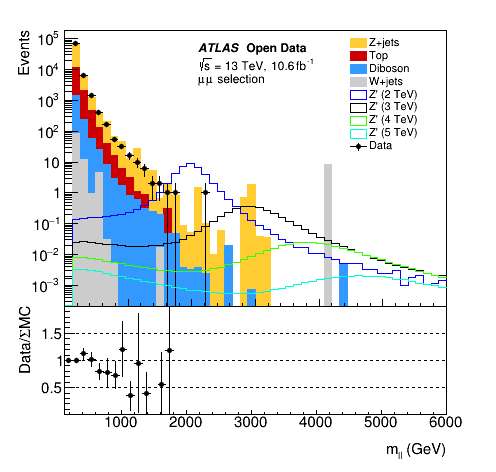
\includegraphics[width=1\linewidth]{uu_mll.png}
%   \caption{1b}
%   \label{fig:uu_mll_6TeV}
% \end{subfigure}
% \caption{plots of....}
% \label{fig:m_ll_6TeV}
% \end{figure}
% \restoregeometry

\begin{figure}[H]
    \begin{center}
        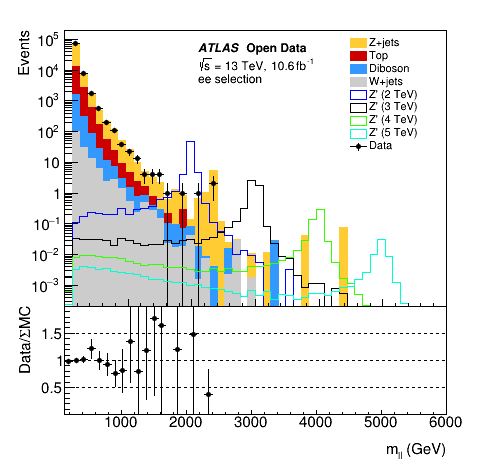
\includegraphics[scale=0.42]{ee_mll.png}
        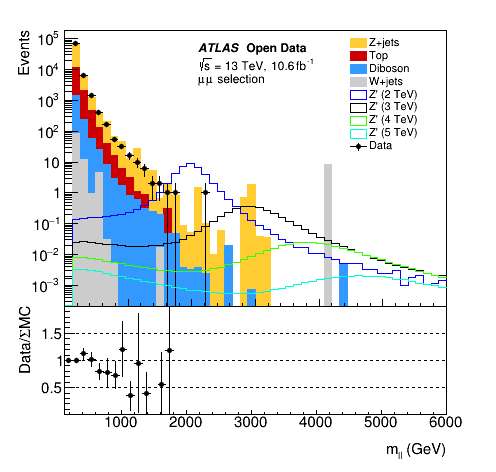
\includegraphics[scale=0.42]{uu_mll.png}
        \caption{The upper panels show histograms of the simulated background and signal (scaled to our data) as well as our data for the $e\bar{e}$ and $\mu \bar{\mu}$ channels. The events are binned according the invariant mass of the leptons. The lower panel shows the data to background ratio to see more clearly how much the data deviates from background.}
        \label{fig:ee_mll_6TeV}
     \end{center}
\end{figure}

% As seen in figure \ref{fig:ee_m_ll_6TeV}, the background is practically zero in the resonance region of both the 4 TeV and 5 TeV Z'. When the background is zero, we can exclude only signals of strengths $s_{up} = -\ln 0.05 \approx 3$ or higher. 

This was done separately for each Z' mass, as the peak will shift with the mass. From figure \ref{fig:ee_mll_6TeV}, it's apparent that we only have data for dilepton invariant masses up to about \SI{2400}{\giga\eV}, which is enough to contain most of the $\SI{2}{\tera \eV}$ peak in addition to a substantial part of the $\SI{3}{\tera \eV}$ signal. Cuts are therefore made on these signals and single-bin estimates for the exclusion limits are made, as will be described in the upcoming subsection. 

\subsection{Exclusion limits}
The $\SI{4}{\tera \eV}$ and  $\SI{5}{\tera \eV}$ signals have peaks far outside our region of data. Being that their signal yield in the data region is extremely small, an optimal cut on these signals would be likely to contain no data. As mentioned in \ref{sec:Bayes}, this means we can only exclude theories which predict signal strengths of $s_{up} = -\ln 0.05 \approx 3$ or higher. Since the predicted $\SI{4}{\tera \eV}$ and  $\SI{5}{\tera \eV}$ signals lie below this limit in both channels, we can not exclude these $Z'$ masses.

Because the simulated background is very small above our data region\footnote{Meaning in the region above $m_{ll} = \SI{2400}{\giga \eV}$.}, we make cuts on the $\SI{2}{\tera \eV}$ and $\SI{3}{\tera \eV}$ signals based on a single $m_{ll}$ value and count everything above this value into one bin. To determine where to cut, the expected exclusion limit\footnote{That is to say the mean exclusion limit with respect to background variations.} was calculated for 9 cut values ranging from \SI{1900}{\giga \eV} to \SI{1100}{\giga \eV} at intervals of \SI{100}{\giga \eV}. For the reasons described in subsection \ref{sec:histogram_cuts}, we opt for the cut that gives the smallest expected exclusion limit. However, cuts that that satisfy: $(\text{observed limit}/{\text{step}) \not\in [100, 1000]$ are excluded to ensure a good interval. 

\begin{figure}[H]
    \begin{center}
        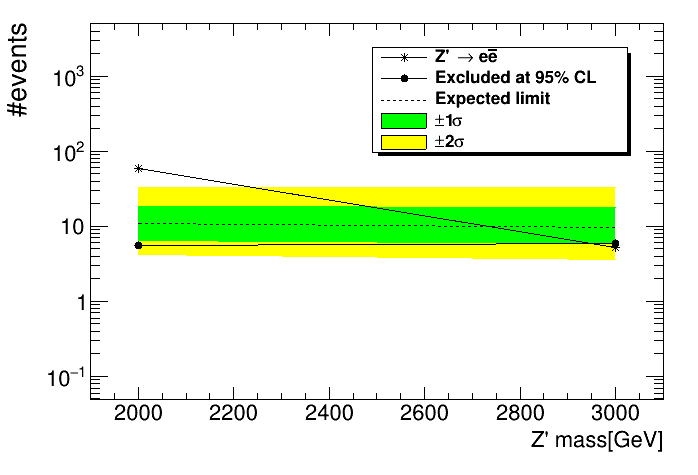
\includegraphics[scale=0.3]{ee_masses.png}
        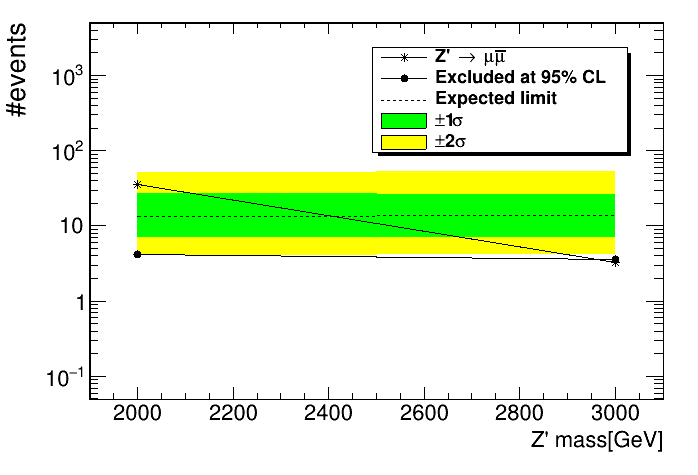
\includegraphics[scale=0.3]{uu_masses.png}
        \caption{Exclusion limits for the $ee$ and $\mu \mu $ channels individually. The line associated with stars show the number of expected signal events (simulated). As can be seen, this line crosses the exclusion line at about 2950 GeV for both channels. Signals corresponding to Z' with masses below this limit can therefore be excluded at 95\% CL.  }
        \label{fig:exclusion_limits}
     \end{center}
\end{figure}

After finding the optimal cuts for the relevant Z' masses in the electron and muon channel, we calculate their exclusion limits $s_{up}$, which are shown as the black dots as seen in figure \ref{fig:exclusion_limits}. Table \ref{tab:exclusion_bands} show the exact values of the exclusion limits and the exclusion bands. The bin-counts are given in table \ref{tab:bin_counts}



\vspace{5mm}




\begin{table}[h!]
\caption{Numerical values of the exclusion limits and exlusion bands shown in figure \ref{fig:exclusion_limits}.}
\label{tab:exclusion_bands}
\centering
% \begin{ruledtabular}
\begin{tabular}{ccc|cccccc}
\hline
\hline
$m_{Z'}[GeV]$ & $m_{ll_{min}}[GeV]$  & Channel & $s_{up}$ & $-2\sigma$ & $-\sigma$ & median &  $+2\sigma$ & $+\sigma$  \\
\hline
\hline

\multirow{2}{*}{2000} &1700 &$e\bar{e}$ & 5.60 & 4.20 & 6.37 & 10.86 & 18.12 & 31.40 \\
                      &1700 & $\mu\Bar{\mu}$ & 4.23 & 4.90 & 7.15 & 13.37 & 26.70 & 51.58 \\
\hline
\multirow{2}{*}{3000} &1900 & $e\bar{e}$ & 5.94 & 3.64 & 5.94 &  9.60& 18.04 & 32.51 \\
                      &1900 & $\mu\Bar{\mu}$ &3.64 & 4.30& 7.33 & 13.78&  26.21 & 51.26 \\

\hline
\hline
\end{tabular}
% \end{ruledtabular}
\end{table} 


\begin{table}[h!]
\caption{Optimal single-bin cuts for the different $m_{Z'}$ masses in both channels and their bin counts. The error in the signal and background counts are given by the ROOT function hist.IntegralAndError().}
\label{tab:bin_counts}
\centering
\begin{tabular}{ccc|cccc}
\hline
\hline
$m_{Z'}[GeV]$ & $m_{ll_{min}}[GeV]$  & Channel & $N_{sig}$ & $N_{bkg}$ & $N_{obs}$  \\
\hline
\hline

\multirow{2}{*}{2000} &1700 &$e\bar{e}$ & 58.59 $\pm$ 0.55 & 9.67 $\pm$ 5.48 & 4 \\
                      &1700 & $\mu\Bar{\mu}$ & 35.60 $\pm$ 0.06 & 13.51 $\pm$ 9.31 &2 \\
\hline
\multirow{2}{*}{3000} &1900 & $e\bar{e}$ & 5.25 $\pm$ 0.05 & 8.33 $\pm$ 5.43 & 4 \\
                      &1900 & $\mu\Bar{\mu}$ & 3.28 $\pm$ 0.005 & 12.67 $\pm$ 9.30 & 1 \\

\hline
\hline
\end{tabular}
\end{table}


Strangely, the exclusion limits lie in the $-2\sigma$ bands. When a single exclusion limit deviates this much from the expected limit, it usually indicates a statistical fluke in the generated background for this particular mass limit. However, all our exclusion limits lie in the $-2\sigma$ bands. Admittedly we have very few data points for the $Z'$ mass, but even so, this should be a very unlikely occurrence. It may be that our event selection is sub-optimal or that there is something that was not accounted for in the code. 

For completeness, we also include the produced histograms of the missing transverse energy and the transverse momentum of the leading lepton. The missing transverse energy is a parameter of interest when there are neutrinos involved in the search process, as is the case in the search for the $W'$ boson. The transverse momentum is of interest, as leptons with very high transverse momenta are likely to be the decay products of heavy particles such as the $Z'$ and $W'$ bosons. Histograms of the mentioned parameters are shown in figure 4 and 5 respectively.




\begin{figure}[h]\label{fig:missing_Et}
    \begin{center}
        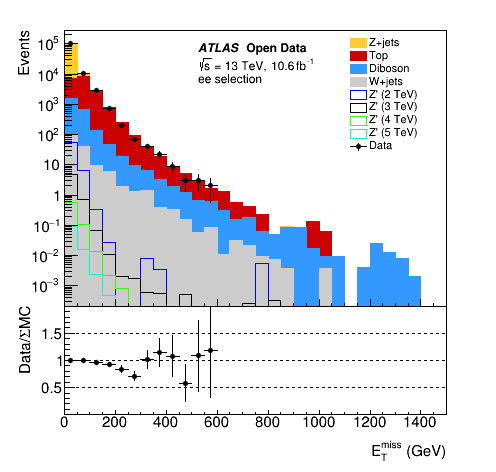
\includegraphics[scale=0.42]{ee_met.png}
        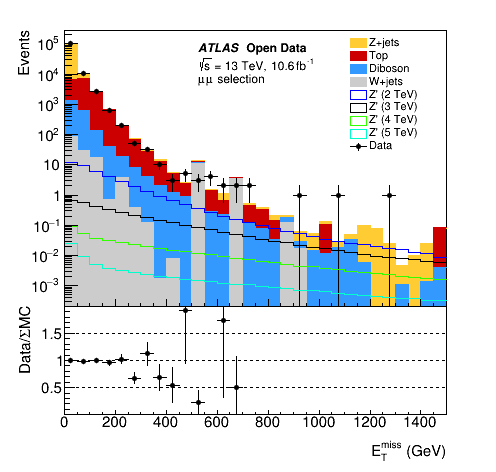
\includegraphics[scale=0.42]{uu_met.png}
        \caption{Missing transverse energy for the leptons in both channels.}
        \label{fig:ee_mll_6TeV}
     \end{center}
\end{figure}

\begin{figure}[h]\label{fig:leading_pt}
    \begin{center}
        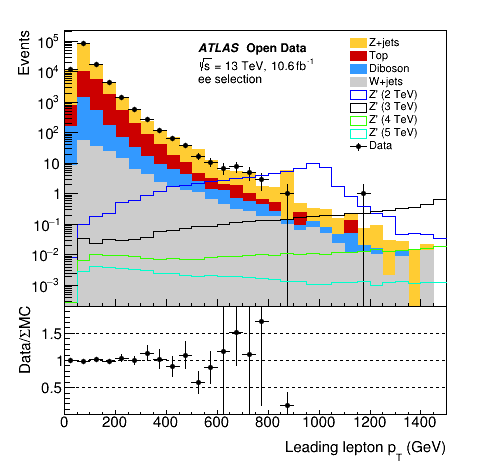
\includegraphics[scale=0.42]{ee_pt1.png}
        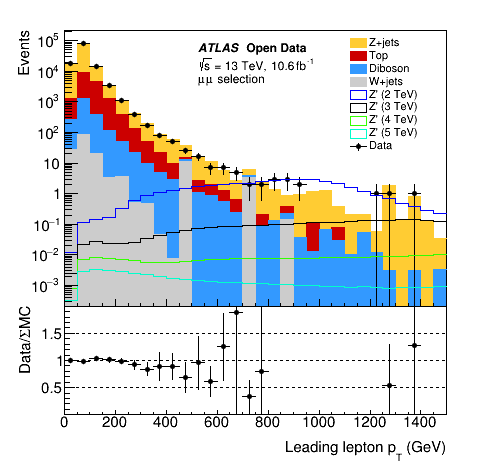
\includegraphics[scale=0.42]{uu_pt1.png}
        \caption{Transverse momenta of the leading leptons for both channels.}
        \label{fig:ee_mll_6TeV}
     \end{center}
\end{figure}







% This is an atrocious act because of the large "background" we would be dealing with. As the background increases, so does the uncertainty of the simulated background in terms of number of events. The expected number of events for the Z' resonance peak remains fixed, and th

% \section{From ATLAS data to exclusion limits}

% The ATLAS data are stored in so-called NTuples, which are TTrees which can only store data as float. 
% For a given dataset, ours being that containing two or more leptons, each possible background channel (in addition to the signal) are stored in a separate NTuple. This means that every useful parameter of a given channel e.g. transverse momentum, pseudorapidity, missing transverse momentum etc. are stored in its own designated leaf within the NTuple. Each branch of the NTuple leads one leaf which contain every measurement of a given feature for a certain channel, stacked on top of each other according to which particular event/entry they belong to. 

% And so a certain event will be stored in a given NTuple and its measured features will be stacked in their corresponding leaves. The set of features for an event across all leaves of a TTree are what we refer to as an entry.

% The next main step is to further reduce the background by excluding entries/events that we can be reasonably certain do not step from the $Z'-> l\Bar{l}$ decay. This is done by MySelector.C, which imposes that the criteria described in section \ref{sec:event_selection} be met. It then goes on to create histograms of each channel with the events that passed the selection criteria. 

% A histogram file contain histograms of each feature of a channel. The next step is to produce the histograms of figure (). We decide on which background channels contribute the most, and list all the dataset ID's of the corresponding TTrees, which are now stored in their respective histogram file. For each background channel, we go through the relevant histogram files and we increment the bins of the final histogram according to the number of entries in the leaf/feature of interest and the their corresponding feature value. The same is done for signal and data. Now we have produced the final histograms. 

% By picking our bins

% This is done by MakePlots.py, and in the case of the 

% count the number of entries stored in all the leaf corresponding to the feature we wish to plot and increment 
% pick the most relevant background channels and for each feature/variable we're interested in, plot 
% combine their In order to produce the histogram plots in figures ..., we need to 



% \begin{figure}[H]
%     \begin{center}
%         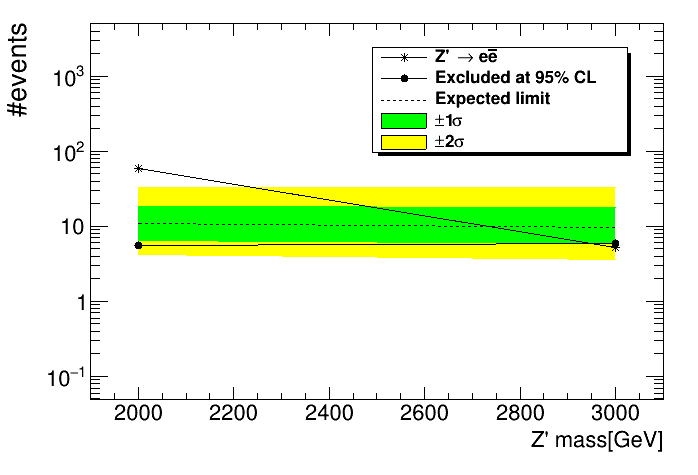
\includegraphics[width=\textwidth]{ee_masses.png}
%         \caption{Atmospheric pressure measured by the each of the POLA detectors for the duration of the PolarqEEEst expedition (July 22 - September 5, 2018)}
%         \label{fig:1}
%      \end{center}
% \end{figure}

% \begin{figure}[H]
%     \begin{center}
%         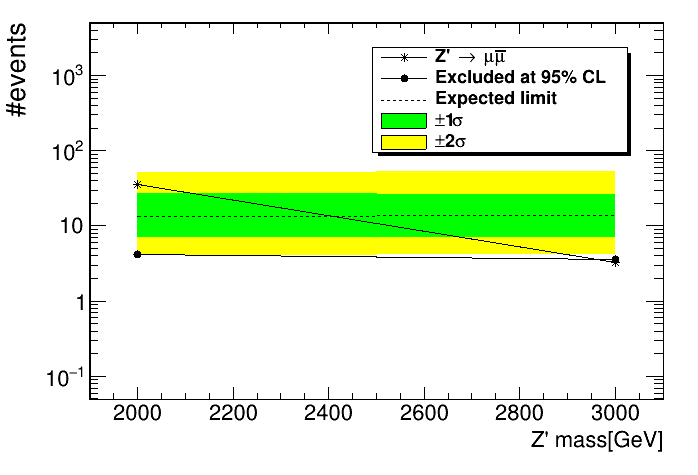
\includegraphics[width=\textwidth]{uu_masses.png}
%         \caption{Atmospheric pressure measured by the each of the POLA detectors for the duration of the PolarqEEEst expedition (July 22 - September 5, 2018)}
%         \label{fig:1}
%      \end{center}
% \end{figure}

\section{Discussion}

In our analysis, we saw that the number of observed events closely matched the background and we got a large deficit in observed events compared to the expected signal yields. The focus was therefore on finding exclusion limits, which we did through Bayesian inference. Had we seen an unexpected high number of events compared with background, we could have calculated the statistical significance of our single bins. This is a frequentist notion, as it relies on the concept of a background hypothesis which the Bayesian formulation does not have. Regardless, it is common practice to use statistical significance when claiming discoveries, although a Bayesian equivalent probably has been formulated. 

Significance is defined based on the probability of observing the number of events we observed under the background hypothesis alone. Specifically, it calculates the area of the likelihood function where $n>n_{obs}$. The smaller this area, the less likely it is to observe $n_{obs}$ under the background hypothesis. Where this area starts can be specified by how many standard deviations $\sigma$ it is from the mean, and this is what we call the significance. 

All four calculated exclusion limits lie in the $-2\sigma$ band. The measurements may therefore be inaccurate, perhaps due to a fault in the code.
% \begin{enumerate}
%     \item We are interested in $p_T$ because a $z'$ decay will produce very high $p_T$ muons and electrons due to its high mass. 
% \end{enumerate}

\printbibliography

\end{document}
